% !TEX root = ./main.tex
\graphicspath{{figures_manufactured/}}% Set graphics path location


\subsection{Method of Manufactured Solutions}
\begin{table}[H]
\centering
\begin{tabular}{ c c c c c c c c} 
  
 Mesh: &   & 4x4 & 8x8 & 16x16 & 32x32 & 64x64 & Overall Order \\ 
 \hline 
 \multirow{2}{*}{$p = 1$} & $L_2$ error & 7.92e-01 & 1.84e-01 & 4.36e-02 & 1.07e-02 & 2.68e-03 &   \\ 
  
   & $\mathcal{O}(L_2)$ &   & 2.10 & 2.08 & 2.03 & 2.00 & 2.05 \\ 
 \hline 
 \multirow{2}{*}{$p = 2$} & $L_2$ error & 1.29e-01 & 1.61e-02 & 1.95e-03 & 2.33e-04 & 2.86e-05 &   \\ 
  
   & $\mathcal{O}(L_2)$ &   & 3.00 & 3.05 & 3.06 & 3.03 & 3.04 \\ 
 \hline 
 \multirow{2}{*}{$p = 3$} & $L_2$ error & 1.01e-02 & 9.25e-04 & 5.71e-05 & 3.65e-06 & 2.35e-07 &   \\ 
  
   & $\mathcal{O}(L_2)$ &   & 3.45 & 4.02 & 3.97 & 3.96 & 3.88 \\ 
 \hline 
 \multirow{2}{*}{$p = 4$} & $L_2$ error & 2.60e-03 & 6.33e-05 & 2.00e-06 & 6.49e-08 & 3.62e-09 &   \\ 
  
   & $\mathcal{O}(L_2)$ &   & 5.36 & 4.98 & 4.95 & 4.16 & 4.88 \\ 
 \hline 
 \multirow{2}{*}{$p = 5$} & $L_2$ error & 7.15e-05 & 3.87e-06 & 6.31e-08 &   &   &   \\ 
  
   & $\mathcal{O}(L_2)$ &   & 4.21 & 5.94 &   &   & 5.07 \\ 
 \hline 
 \end{tabular}
\caption{Tris} 
 \end{table}


\begin{figure}
\centering
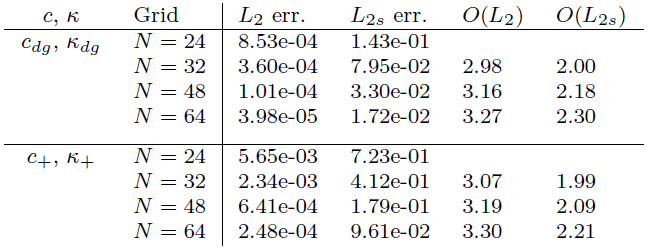
\includegraphics[height=35mm]{table_917} \\
\caption{Accuracy of ESFR schemes for flow generated by a time-dependent source term on triangular grids, for the case of $p = 2$. The inviscid and viscous numerical fluxes were computed using a Rusanov flux with $\lambda = 1$ and a LDG flux with $\tau = 0.1$ and $\beta = \pm 0.5n$.}
\label{fig:table_917}
\end{figure}

\begin{figure}
\centering
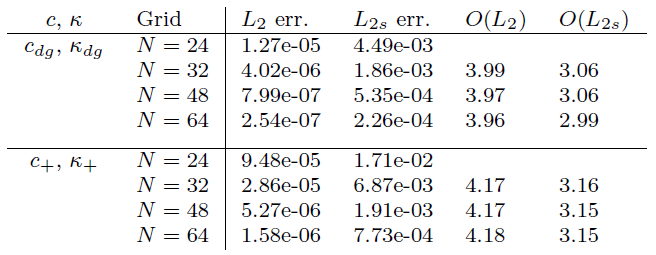
\includegraphics[height=35mm]{table_918} \\
\caption{Accuracy of ESFR schemes for flow generated by a time-dependent source term on triangular grids, for the case of $p = 3$. The inviscid and viscous numerical fluxes were computed using a Rusanov flux with $\lambda = 1$ and a LDG flux with $\tau = 0.1$ and $\beta = \pm 0.5n$.}
\label{fig:table_918}
\end{figure}

\begin{figure}
\centering
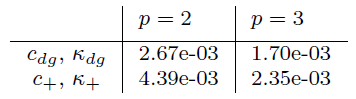
\includegraphics[height=20mm]{table_919} \\
\caption{Explicit time-step limits ($\Delta t_{max}$) of ESFR schemes for flow generated by a time-dependent source term on the triangular grid with $\tilde{N} = 48$, for the cases of $p = 2$ and $3$. The inviscid and viscous numerical fluxes were computed using a Rusanov flux with $\lambda = 1$ and a LDG flux with $\tau = 0.1$ and $\beta = \pm 0.5n$.}
\label{fig:table_919}
\end{figure}

\begin{figure}
\centering
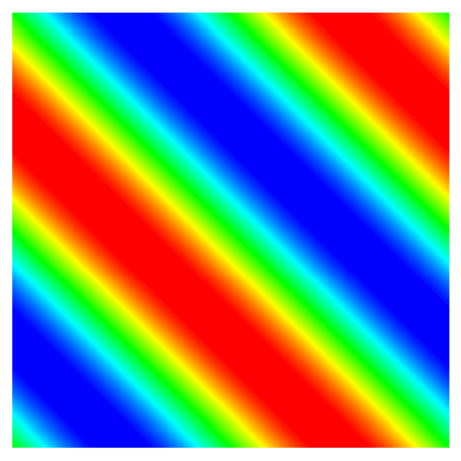
\includegraphics[height=60mm]{figure_912} \\
\caption{Contours of energy obtained using the ESFR scheme with $c = c_+$ and $\kappa = \kappa_+$ on the triangular grid with $\tilde{N} = 32$ for the case of $p = 3$. The inviscid and viscous numerical fluxes were computed using a Rusanov flux with $\lambda = 1$ and a LDG flux with $\tau = 0.1$ and $\beta = \pm 0.5n$.}
\label{fig:figure_912}
\end{figure}

\begin{figure}
\centering
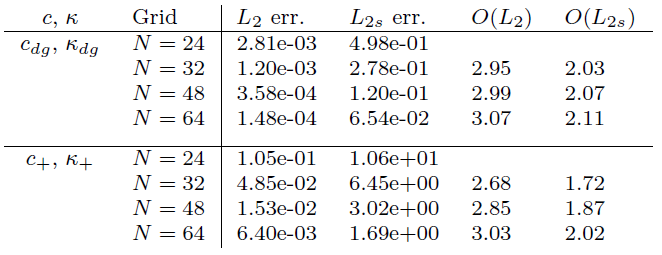
\includegraphics[height=35mm]{table_920} \\
\caption{Accuracy of ESFR schemes for flow generated by a time-dependent source term on tetrahedral grids, for the case of $p = 2$. The inviscid and viscous numerical fluxes were computed using a Rusanov flux with $\lambda = 1$ and a LDG flux with $\tau = 0.1$ and $\beta = \pm 0.5n$.}
\label{fig:table_920}
\end{figure}

\begin{figure}
\centering
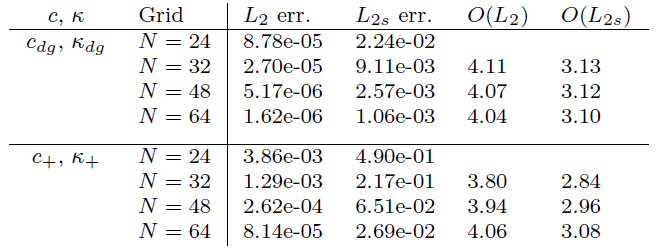
\includegraphics[height=30mm]{table_921} \\
\caption{Accuracy of ESFR schemes for flow generated by a time-dependent source term on tetrahedral grids, for the case of $p = 3$. The inviscid and viscous numerical fluxes were computed using a Rusanov flux with $\lambda = 1$ and a LDG flux with $\tau = 0.1$ and $\beta = \pm 0.5n$.}
\label{fig:table_921}
\end{figure}

\begin{figure}
\centering
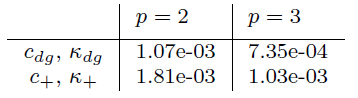
\includegraphics[height=15mm]{table_922} \\
\caption{Explicit time-step limits ($\Delta t_{max}$) of ESFR schemes for flow generated by a time-dependent source term on the triangular grid with $\tilde{N} = 48$, for the cases of $p = 2 and 3$. The inviscid and viscous numerical fluxes were computed using a Rusanov flux with $\lambda = 1$ and a LDG flux with $\tau = 0.1$ and $\beta = \pm 0.5n$.}
\label{fig:table_922}
\end{figure}

\newpage
\begin{figure}
\centering
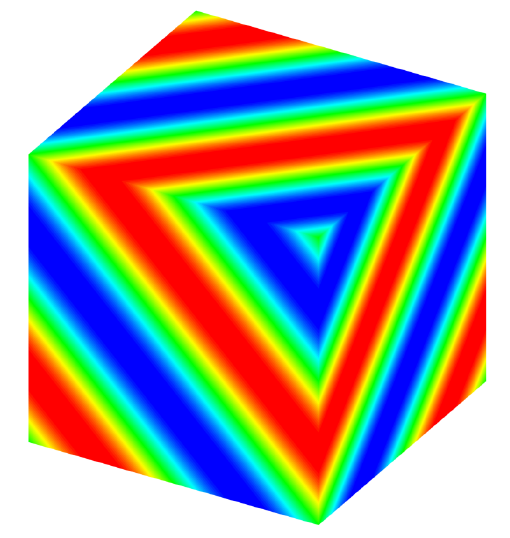
\includegraphics[height=60mm]{figure_913} \\
\caption{Contours of energy obtained using the ESFR scheme with $c = c_+$ and $\kappa = \kappa_+$ on the tetrahedral grid with $\tilde{N} = 32$ for the case of $p = 3$. The inviscid and viscous numerical fluxes were computed using a Rusanov flux with $\lambda = 1$ and a LDG flux with $\tau = 0.1$ and $\beta = \pm 0.5n$.}
\label{fig:figure_913}
\end{figure}
